\documentclass[11pt]{article}
\usepackage[margin=0.80in, paperwidth=8.5in, paperheight=11in]{geometry}
\usepackage{amsfonts}
\usepackage{amsmath}
\usepackage{amssymb}
\usepackage{bm}
\usepackage{authblk}
\usepackage{graphicx}
\usepackage{listings}
\usepackage{array}
\usepackage{booktabs}
\usepackage{titlesec}
\usepackage{pgfplotstable}\pgfplotsset{compat=1.13}

\newcommand{\bs}[1]{\boldsymbol{#1}}
\newcommand{\del}[2]{\frac{\partial {#1}}{\partial {#2}}}
\newcommand{\dv}[3]{\frac{{\rm d}^{#1}{#2}}{d{#3}^{#1}}}
\newcommand{\ddel}[2]{\frac{\partial^2 {#1}}{\partial {#2}^2}}
\newcommand{\dev}{{\rm {\bf dev}}}
\newcommand{\proj}[1]{\frac{1}{R^2}{\bf X}\otimes{\bf X}}
\newcommand{\Ie}[1]{I^{\rm e}_{#1}}
\newcommand{\Ce}[1]{\bf C^{\rm e^{#1}}}
\newcommand{\Fe}[2]{F^{\rm e^{#2}}_{#1}}
\newcommand{\Fv}[2]{F^{\rm v^{#2}}_{#1}}
\newcommand{\f}[2]{f^{\rm {#2}}_{#1}}
\newcommand{\fv}[2]{f^{\rm v^{#2}}_{#1}}
\newcommand{\dfv}[2]{\dot{f}^{\rm v^{#2}}_{#1}}
\newcommand{\tGam}[2]{\tilde{\Gamma}^{\rm v^{#2}}_{#1}}
\newcommand{\Gam}[2]{\Gamma^{\rm v^{#2}}_{#1}}
\newcommand{\A}[1]{\mathcal{A}_{#1}}
\newcommand{\F}[2]{F^{\rm #2}_{#1}}
\newcommand{\hpeq}{\hat{\psi}^{\rm Eq}}
\newcommand{\hpneq}{\hat{\psi}^{\rm NEq}}
\newcommand{\etak}{\eta_K({I_1,I_2,J},{\bf C^{\rm e}, B^{\rm v}})}
\newcommand{\nuk}{\nu_K({I_1,I_2,J},{\bf C^{\rm e}, B^{\rm v}})}
\newcommand{\thetak}{\theta_K({I_1,I_2,J},{\bf C^{\rm e}, B^{\rm v}})}
\newcommand{\etaj}{\eta_J({I_1,I_2,J},{\bf C^{\rm e}, B^{\rm v}})}
\newcommand{\dFv}[2]{\dot{F}^{\rm v^{#2}}_{#1}}
\newcommand{\hatpsi}{\widehat{\psi}(I_1, I_2,I^{\rm e}_1,I^{\rm e}_2,J)}
\newcommand{\hpsi}{\widehat{\psi}(I_1,I^{\rm e}_1,J)}
\newcommand{\Fh}[1]{\widehat{\mathcal{F}}\left({\bf F, \Fv{}{}}, {#1}\right)}
\newcommand{\Fhstar}[1]{\widehat{\mathcal{F}}^*\left({\bf F, \Fv{}{}}, {#1}\right)}
\newcommand{\sbar}{\overline{\bm{\sigma}}}
\newcommand{\hpsicomp}[1]{\sum_{r=1}^{2}\left\{\frac{3^{1-\alpha_r}}{2\alpha_r}\mu_r(I^{\alpha_r}_1-3^{\alpha_r})
+\frac{3^{1-a_r}}{2a_r}m_r({\Ie{1}}^{^{a_r}}-3^{a_r})\right\}
+\mu{#1}+\kappa{#1}^2}
\newcommand{\Ni}[1]{N^{(e)}_i(#1)}
\newcommand{\hNi}[1]{\hat{{N}}^{(e)}_i(#1)}

\titlespacing\section{10pt}{14pt plus 4pt minus 2pt}{10pt plus 2pt minus 2pt}
\titlespacing\subsection{0pt}{12pt plus 4pt minus 2pt}{8pt plus 2pt minus 2pt}
\titlespacing\subsubsection{0pt}{12pt plus 4pt minus 2pt}{6pt plus 2pt minus 2pt}
\usepackage{color} %red, green, blue, yellow, cyan, magenta, black, white
\definecolor{mygreen}{RGB}{28,172,0} % color values Red, Green, Blue
\definecolor{mylilas}{RGB}{170,55,241}
\graphicspath{{Figures/}}
\title{\bf CEE 576: Nonlinear Finite Elements - Fall 2016 \\ Homework 2}
\author{Bhavesh Shrimali (NetID: bshrima2)}
\begin{document}
\maketitle \hrule \hrule \hrule
\section*{Sol$^{\rm n}$ 1:}
The general nonlinear finite element formulation for 3-D Elasticity problem can be described as follows: 
\begin{align}
a
\left({\bf w},{\bf u};{\bf u},{\bf x}
\right)
=
({\bf w},{\bf f})_{_{\Omega}}
+
({\bf w},{\bf h})_{_{\Gamma_h}}
\label{Eqn1}
\end{align}
where 
\[
a
\left({\bf w},{\bf u};{\bf u},{\bf x}
\right)
 = \int_{\Omega} w_{i,j} \sigma_{ij} \left( \epsilon_{ij},{\bf x} \right) \ d \Omega\ ; \ \ \ \ \ 
 ({\bf w},{\bf f})_{_{\Omega}} = \int_{\Omega} w_i f_i \ d \Omega\ ; \ \ \ \ \ ({\bf w},{\bf h})_{_{\Gamma_h}} = \int_{\Gamma_h} w_i h_i\ d\Gamma
\]
The corresponding 1-D version of Equation (\ref{Eqn1}) be stated as follows: 
\[
a(w,u;u,x) = (w,f)_{_{\Omega}} + (w,h)_{_{\Gamma}}
\]
The Galerkin form is similar to the above equation, except that the functions $w^h$, $u^h$ and $f^h$ are piece-wise continuous over each element. Moreover $f^h$ can be thought of as the mapping of the forcing function of the finite element space of functions. 
\begin{align}
a(w^h,u^h;u^h, x) = \int_{\Omega} w^h_{,x} \sigma^h \left( u^h_{,x} \right); \ \ \ \ \ (w^h,f^h)_{\Omega} = \int_{\Omega} w^h f^h\ d\Omega \ ; \ \ \ \ (w^h,h) = \int_{\Gamma_h} w^h h \ d\Gamma 
\end{align}
\subsection*{(a) Strong Form (S):}
For the nonlinear 1D elasticity problem, given external forcing function $f(x)$ and material parameters $\left\{\Omega = (0,1)\right\}$, find $u(x): \Omega \rightarrow \mathbb{R}$ such that $u(x) \in \mathcal{U}$ and 
\begin{align}
\begin{split}
\sigma,_{x} \left(u,_{x}; x \right) + f(x) = 0 \\
u(1) = g; \ \ \ \ \ \sigma(0) = h
\end{split}
\label{StrongForm}
\end{align}
where
\[
\mathcal{U} =  \left\{ u(x)\ | \ u(x) \in C^2 \left( 0,1 \right), u(1) = g \right\} 
\]
The dependence on $x$ (inhomogeneity) appears in the first term in the expression, which ultimately appears in the Consistent-tangent tensor. The forcing function $f(x)$ may (or may not) potentially depend on the spatial variable $x$. \\ \hrule
\subsection*{(b) Weak Form (W):}
We multiply Equation(\ref{StrongForm})$_1$ by a test function $w(x)$ and integrate by parts to get 
\[
\int_{\Omega} w,_{x}(x) \sigma\left(u,_{x}; x \right)\ d\Omega =  w(x)\sigma\left(u,_{x}; x \right) |_{\Gamma_h} + \int_{\Omega} w(x) f(x)\ d\Omega
\]
Thus the Weak form (W) can be stated as follows: \\ \noindent Given $f(x)$ and other material parameters $\left\{\Omega = (0,1)\right\}$, find $u(x): \Omega \rightarrow \mathbb{R}$ such that $u(x) \in \mathcal{U}_0 (\Omega)$
\begin{align}
\int_{\Omega} w,_{x}(x) \sigma\left(u,_{x}; x \right)\ d\Omega =  w(x)\sigma\left(u,_{x}; x \right) |_{\Gamma_h} + \int_{\Omega} w(x) f(x)\ d\Omega \ \ \ \ \ \ \ \forall w(x) \in \mathcal{V}(\Omega)
\end{align}
\begin{align*}
\mathcal{U}_0(\Omega) &= \left\{ u\ | u(x) \in {\bf{H}}^1 (\Omega),\ u(x)_{|_{\Gamma_g}} = g\right\}\\
\mathcal{V}(\Omega) & = \left\{ w\ | w(x) \in {\bf{H}}^1 (\Omega),\ w(x)_{|_{\Gamma_g}} = 0\right\}
\end{align*} \hrule
\subsection*{(c) Galerkin-Form (G):}
We now introduce the concept of discretization (mesh). The Galerkin-form (G) is, find $u^h(x): \Omega_e \rightarrow \mathbb{R}$ such that $u^h(x) \in \mathcal{U}^h_0 (\Omega_e)$
\begin{align}
\sum_{e=1}^{n_{el}}\int_{\Omega_e} w^h,_{x}(x)\ \sigma\left(u^h,_{x}; x \right)\ d\Omega =  w^h(x)\sigma\left(u^h,_{x}; x \right) |_{\Gamma_h} + \sum_{e=1}^{n_{el}}\int_{\Omega_e} w^h(x) f^h(x)\ d\Omega \ \ \ \ \ \ \ \forall w^h(x) \in \mathcal{V}^h(\Omega_e)
\end{align} 
\begin{align*}
\mathcal{U}^h_0(\Omega_e) &= \left\{ u^h (x)\ | u^h(x) \in {\bf{H}}^1 (\Omega_e),\ u^h(x)_{|_{\Gamma_g}} = g\right\}\\
\mathcal{V}^h(\Omega_e) & = \left\{ w^h(x)\ | w^h(x) \in {\bf{H}}^1 (\Omega_e),\ w^h(x)_{|_{\Gamma_g}} = 0\right\}
\end{align*}
\subsection*{Choice of Shape Functions:}
For the first part of the problem we consider linear shape functions to compute the external force vector, internal force vector, and consistent tangent i.e. for $-1\leq\xi\leq 1$
\[
N(\xi) 
=\frac{1}{2}
\begin{Bmatrix}
{1-\xi} \\
{1+\xi}
\end{Bmatrix}
\]
For the Part.B and Part.C of the problem, separate reference to quadratic shape functions is made. We use isoparametric elements throughout, and hence \[
{x} = \sum_{i=1}^{n_{en}} N^e_i (\xi) \ x_i
\]  \hrule
\subsection*{(d) Nonlinear Matrix Problem: }
\subsubsection*{1. External Force Vector:}
The external load vector, for an element is calculated as follows:
\begin{align}
\begin{split}
{\bf f}^e_a  & = \int_{\Omega_e} N_a(\xi)\ \hat{f}(x)\ d\Omega \\
& = \int_{\Omega} N_a (\xi) N_b(\xi) f_b\ d\Omega
\end{split}
\end{align}
where $f_b$ represent the nodal values of $f^h (x) $. It can be interpreted as the projection of the actual forcing function on the finite element space of functions used to discretize the field. We use one point Gauss-Quadrature to evaluate the integral
\begin{align*}
\begin{split}
{\bf f}^e_a 
& =
\int_{\Omega_e} {\bf N}^T {\bf N}\ {\bf f}_{\rm nodal} \ d\Omega \\
& = \int_{\Omega_e} \frac{1}{4}
\begin{bmatrix}
\left( 1- \xi \right)^2 & \left( 1- \xi ^2 \right) \\
\left( 1- \xi^2 \right) & \left( 1+ \xi \right)^2 \\
\end{bmatrix} 
\begin{Bmatrix}
f_1 \\
f_2
\end{Bmatrix}\ d\Omega \\
& = \int_{-1}^{1} \frac{1}{4}
\begin{bmatrix}
\left( 1- \xi \right)^2 & \left( 1- \xi ^2 \right) \\
\left( 1- \xi^2 \right) & \left( 1+ \xi \right)^2 \\
\end{bmatrix} 
\begin{Bmatrix}
f_1 \\
f_2
\end{Bmatrix}\ \frac{1}{2}\ d\xi \\ \\
& = \frac{1}{4}
\begin{Bmatrix}
f_1 + f_2 \\
f_1 + f_2
\end{Bmatrix} + 
\begin{Bmatrix}
h\\0
\end{Bmatrix}
\end{split}
\end{align*}
\subsubsection*{2. Internal Force Vector: }
The internal force vector for an element is calculated as follows: 
\begin{align*}
{\bf n}^e_a 
& =
\int_{\Omega_e}
N_a,_{_x} \sigma \left(\epsilon^h; x \right)\ d\Omega \\
\text{where,} \ \ \ \epsilon^h & = u^h,_x (x) = \sum_{e = 1}^{n_{en}} N_e,_{_x} (\xi) \ d_e \\ 
{{\bf n}^e_a} & = \int_{\xi = -1}^{1} \frac{2}{h^e} \frac{1}{2}\begin{Bmatrix} 
-1 \\1
\end{Bmatrix}
\ \sigma \left( \frac{1}{h^e} \left( d^e_2 - d^e_1 \right)\ ;x(\xi)  \right) \frac{h^e}{2}\  d\xi
\end{align*}
Using one point Quadrature ($W = 2$ and $\xi = 0$): 
\begin{align*}
{\bf n}^e_a & = 2 \cdot \frac{1}{2} \begin{Bmatrix}
-1\\1
\end{Bmatrix}
\sigma \left( \frac{1}{h^e} \left( d^e_2 - d^e_1 \right)\ ;\frac{x^e_1 + x^e_2}{2}  \right) \\
& =  
\begin{Bmatrix}
-1\\1
\end{Bmatrix}
\sigma \left( d^e_2 - d^e_1 \ ;\frac{x^e_1 + x^e_2}{2}  \right)
\end{align*}
The Matrix Problem is just $\mathbb{A}^{n_{el}}_{e=1} \ \left\{ {\bf n}^e_a \right\}= \mathbb{A}^{n_{el}}_{e=1} {\bf f}^{e}_a$, where the operator, $\mathbb{A}^{n_{el}}_{e=1}$, is the assembly operator over all elements in the mesh. Thus we get
\begin{align*}
{\bf f}^e_a = \int_{\Omega} {\bf N}_a {\bf N}_b f^{\rm nodal}_b\ d\Omega + {\bf N}_{a_{x= 0}} \cdot h
\end{align*} \hrule
\subsection*{(e) Consistent Tangent Tensor: }
The consistent tangent tensor can be obtained by taking the variational derivative (in this case the Taylor-Expansion) of the internal force vector: 
\begin{align*}
\mathbb{D} {{\bf n}^e_a} & = \del{{\bf n}^e_a}{d_b} \\
& = \del{}{d_b} \int_{\Omega_e}  N_a,_{_x} \sigma \left(\epsilon^h; x \right)\ d\Omega
\end{align*}
Applying the chain-rule of differentiation, with ($h^e = 1$): 
\begin{align}
\begin{split}
& \int_{\Omega_e}  N_a,_{_x} (\xi)\ \del{}{\epsilon^h} \sigma \left(\epsilon^h; x \right) \del{\epsilon^h}{d_b} \ d\Omega \\
& = \int_{\Omega_e}  N_a,_{_x} (\xi)\ \mathbb{C} \left(\epsilon^h; x \right) N_e,_{_x} (\xi)\ \delta_{eb} \ d\Omega \\
& = \int_{\Omega_e}  N_a,_{_x} (\xi)\ \mathbb{C} \left(\epsilon^h; x \right) N_b,_{_x} (\xi) \ d\Omega \\
& = \int_{-1}^{1} \frac{2}{h^e} N_a,_{_\xi} (\xi)\ \mathbb{C} \left( \epsilon^h(\xi);x(\xi) \right) N_b,_{_\xi} (\xi)\ d\xi  \\
& = 2 \cdot 2 \frac{1}{4} 
\begin{Bmatrix}
-1 \\
1
\end{Bmatrix}
\mathbb{C}
\left(
\frac{d^e_2 - d^e_1}{h^e} ; \frac{x^e_2 + x^e_1}{2}
\right)
\begin{Bmatrix}
-1 & 1
\end{Bmatrix}\\ \\
& =  
\begin{bmatrix}
1 & -1 \\
-1 & 1
\end{bmatrix} \mathbb{C}
\left(
{d^e_2 - d^e_1} ; \frac{x^e_2 + x^e_1}{2}
\right)
\end{split}
\label{ConsTang}
\end{align} \hrule
\subsection*{(f) Internal Force:}
For this part, and the next, calculations are presented with respect to quadratic shape functions and 2-point numerical quadrature. 
\subsubsection*{Choice of Shape Functions:}
1-D Quadratic Shape Functions, listed for the given element as shown in the figure:
\[
N\left( \xi \right) = \frac{1}{2}
\begin{Bmatrix}
\xi (\xi -1 )  \\
2 (1+\xi) (1-\xi)\\
\xi (\xi+1)
\end{Bmatrix}
\]
\begin{center}
Assumption: The internal node is equidistant from the other two nodes. 
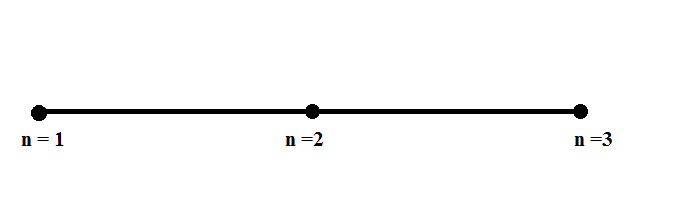
\includegraphics[scale=1]{fig}
\end{center}
\newpage
\subsubsection*{Calculations: }
\begin{align}
{\bf n}^e_a 
& =
\int_{\Omega_e}
N_a,_{_x} \sigma \left(\epsilon^h; x \right)\ d\Omega 
\end{align}
Again using isoparametric elements: 
\[
{x} = \sum_{i=1}^{n_{en}} N^e_i (\xi) \ x_i
\]
Thus 
\[
J = \dv{}{x}{\xi} = \sum_{i=1}^{n_{en}} \dv{}{N^e_i}{\xi} (\xi) \ x^e_i = \frac{(2\xi -1)}{2}x^e_1 -2\xi x^e_2 + \frac{(2\xi + 1)}{2}x^e_3 =  \frac{1}{2}
\]
\begin{align*}
{\bf n}^e_a 
=
\int_{-1}^{1} \frac{1}{2}
\begin{bmatrix}
2\xi - 1 \\ -4\xi \\ 2\xi+1
\end{bmatrix} \sigma \left(\epsilon^h(\xi); x(\xi) \right)\ d\xi
\end{align*}
Now using 2-point Gauss-Quadrature to integrate the above polynomial, we get: 
\begin{align}
\begin{split}
& \frac{1}{2}\begin{bmatrix}
2\xi - 1 \\ -4\xi \\ 2\xi+1
\end{bmatrix} \sigma \left(\epsilon^h(\xi); x(\xi) \right) \Bigr|_{\substack{\xi = -\frac{1}{\sqrt{3}}}} 
+ 
\frac{1}{2}\begin{bmatrix}
2\xi - 1 \\ -4\xi \\ 2\xi+1
\end{bmatrix} \sigma \left(\epsilon^h(\xi); x(\xi) \right) \Bigr|_{\substack{\xi = \frac{1}{\sqrt{3}}}} \\ \\
& = \begin{bmatrix}
-1.07735 \\ 1.155 \\ -0.07735
\end{bmatrix} \sigma \left(\epsilon^h(\frac{-1}{\sqrt{3}}); x(\frac{-1}{\sqrt{3}}) \right) 
+ \begin{bmatrix}
0.07735 \\ -1.155 \\ 1.07735
\end{bmatrix}\sigma \left(\epsilon^h(\frac{1}{\sqrt{3}}); x(\frac{1}{\sqrt{3}}) \right)
\end{split}
\end{align}
where, 
\[
\epsilon^h \left(\frac{-1}{\sqrt{3}} \right) 
= 
-2.1547 d^e_1 + 2.311 d^e_2 - 0.1547 d^e_3\ ; \ \ \ \ \ \ 
x\left(\frac{-1}{\sqrt{3}} \right) 
= 0.455 x^e_1 + 0.667 x^e_2 -0.122 x^e_3 = 0.2115
\]
\[
\epsilon^h \left(\frac{1}{\sqrt{3}} \right) 
= 
0.1547 d^e_1 - 2.311 d^e_2 + 2.1547 d^e_3\ ; \ \ \ \ \ \ x\left(\frac{1}{\sqrt{3}} \right) 
= -0.122 x^e_1 + 0.667 x^e_2 + 0.455 x^e_3 = 0.7885
\] \\ \hrule 
\subsection*{(g) Consistent Tangent Tensor: }
Using the calculation carried out in (\ref{ConsTang}) we have
\begin{align}
\begin{split}
\mathbb{D}{\bf n}^e_a 
& = 
\int_{-1}^{1} \frac{2}{h^e} N_a,_{_\xi} (\xi)\ \mathbb{C} \left( \epsilon^h(\xi);x(\xi) \right) N_b,_{_\xi} (\xi)\ d\xi  \\
& = \int_{-1}^{1}
\frac{2}{h^e} \frac{1}{4} 
\begin{bmatrix}
2\xi - 1 \\ -4\xi \\ 2\xi + 1 
\end{bmatrix}
\mathbb{C}
\left(
\epsilon^h (\xi) ; x(\xi)
\right)
\begin{bmatrix}
2\xi - 1 & -4\xi & 2\xi + 1 
\end{bmatrix}\ d\xi \\
& = 
\int_{-1}^{1} \frac{1}{2}
\begin{bmatrix}
(2\xi - 1)^2 & -4\xi(2\xi - 1) & 4{\xi}^2 - 1 \\
-4\xi(2\xi - 1) & 16{\xi}^2 & -4\xi(2\xi + 1) \\
4{\xi}^2 - 1 & -4\xi(2\xi + 1) & (2\xi + 1)^2
\end{bmatrix} \mathbb{C}
\left(
\epsilon^h (\xi) ; x(\xi)
\right)\ d\xi
\end{split}  
\end{align}
Using 2-point Gauss-Quadrature to calculate the above integral we get,
\begin{align}
\frac{1}{2}\left[
\begin{bmatrix}
4.642 & -4.976 & 0.333 \\
-4.976 & 5.33 & -0.357 \\
0.333 & -0.357 & 0.0239
\end{bmatrix}\ \mathbb{C}
\left(
\epsilon^h (\frac{-1}{\sqrt{3}}) ; x(\frac{-1}{\sqrt{3}})
\right)+
\begin{bmatrix}
0.0239 & -0.357 & 0.333 \\
-0.357 & 5.33 & -4.976 \\
0.333 & -4.976 & 4.642
\end{bmatrix}\ \mathbb{C}
\left(
\epsilon^h (\frac{1}{\sqrt{3}}) ; x(\frac{1}{\sqrt{3}})
\right)
\right]
\end{align}
Thus the Consistent Tangent Tensor, evaluated using the 2-point Gauss-Quadrature would be as follows: 
\begin{align}
\begin{bmatrix}
2.321 & -2.488 & 0.167 \\
-2.488 & 2.667 & -0.179 \\
0.167 & -0.179 & 0.012
\end{bmatrix}\ \mathbb{C}
\left(
\epsilon^h (\frac{-1}{\sqrt{3}}) ; x(\frac{-1}{\sqrt{3}})
\right)+
\begin{bmatrix}
0.012 & -0.179 & 0.167 \\
-0.179 & 2.667 & - 2.488 \\
0.167 & -2.488 & 2.321
\end{bmatrix}\ \mathbb{C}
\left(
\epsilon^h (\frac{1}{\sqrt{3}}) ; x(\frac{1}{\sqrt{3}})
\right)
\end{align}
where,
\[
\epsilon^h \left(\frac{-1}{\sqrt{3}} \right) 
= 
-2.1547 d^e_1 + 2.311 d^e_2 - 0.1547 d^e_3\ ; \ \ \ \ \ \ 
x\left(\frac{-1}{\sqrt{3}} \right) 
= 0.455 x^e_1 + 0.667 x^e_2 -0.122 x^e_3 = 0.2115
\]
\[
\epsilon^h \left(\frac{1}{\sqrt{3}} \right) 
= 
0.1547 d^e_1 - 2.311 d^e_2 + 2.1547 d^e_3\ ; \ \ \ \ \ \ x\left(\frac{1}{\sqrt{3}} \right) 
= -0.122 x^e_1 + 0.667 x^e_2 + 0.455 x^e_3 = 0.7885
\]  \\ \hrule
\subsection*{Part C.:}
No, 1-point Gauss-Quadrature cannot integrate this problem exactly. 
\begin{itemize}
\item A general $m$-point Quadrature can exactly integrate a polynomial of order $2m-1$, thus 1-point Quadrature can only integrate linear polynomials. 
\item For the consistent tangent tensor there are quadratic polynomials to be integrated (at-least considering {$\mathbb{C}$} remains constant) or higher. 
\item Thus, we would need higher order quadrature, potentially 2 (in case of constant $\mathbb{C}$) or even more depending on the dependance of $\mathbb{C}$ on $x$, to exactly integrate this problem.
\end{itemize}
\subsubsection*{Some remarks about internal force vector:}
\begin{itemize}
\item For the internal force vector, we have linear polynomials to be integrated at least,(if $\sigma$ is constant), but in case of non-homogeneous materials $\sigma(\epsilon;x)$ and hence one point quadrature would not be able to exactly integrate the problem. 
\end{itemize}
\subsubsection*{Some remarks about external force vector:}
\begin{itemize}
\item In case of the external force vector we will have the product of shape functions $N_i N_j$ and the nodal values of the forcing function.
\item This would lead to a biquadratic polynomial and hence, even 2-point Gauss-Quadrature would not be sufficient to exactly integrate the external load vector. 
\end{itemize} \hrule
\newpage 
\section*{Sol$^n$ 2: }
The given problem is solved using the provided Matlab-Code: 
\subsection*{(a) Results: Plots}
\begin{center}
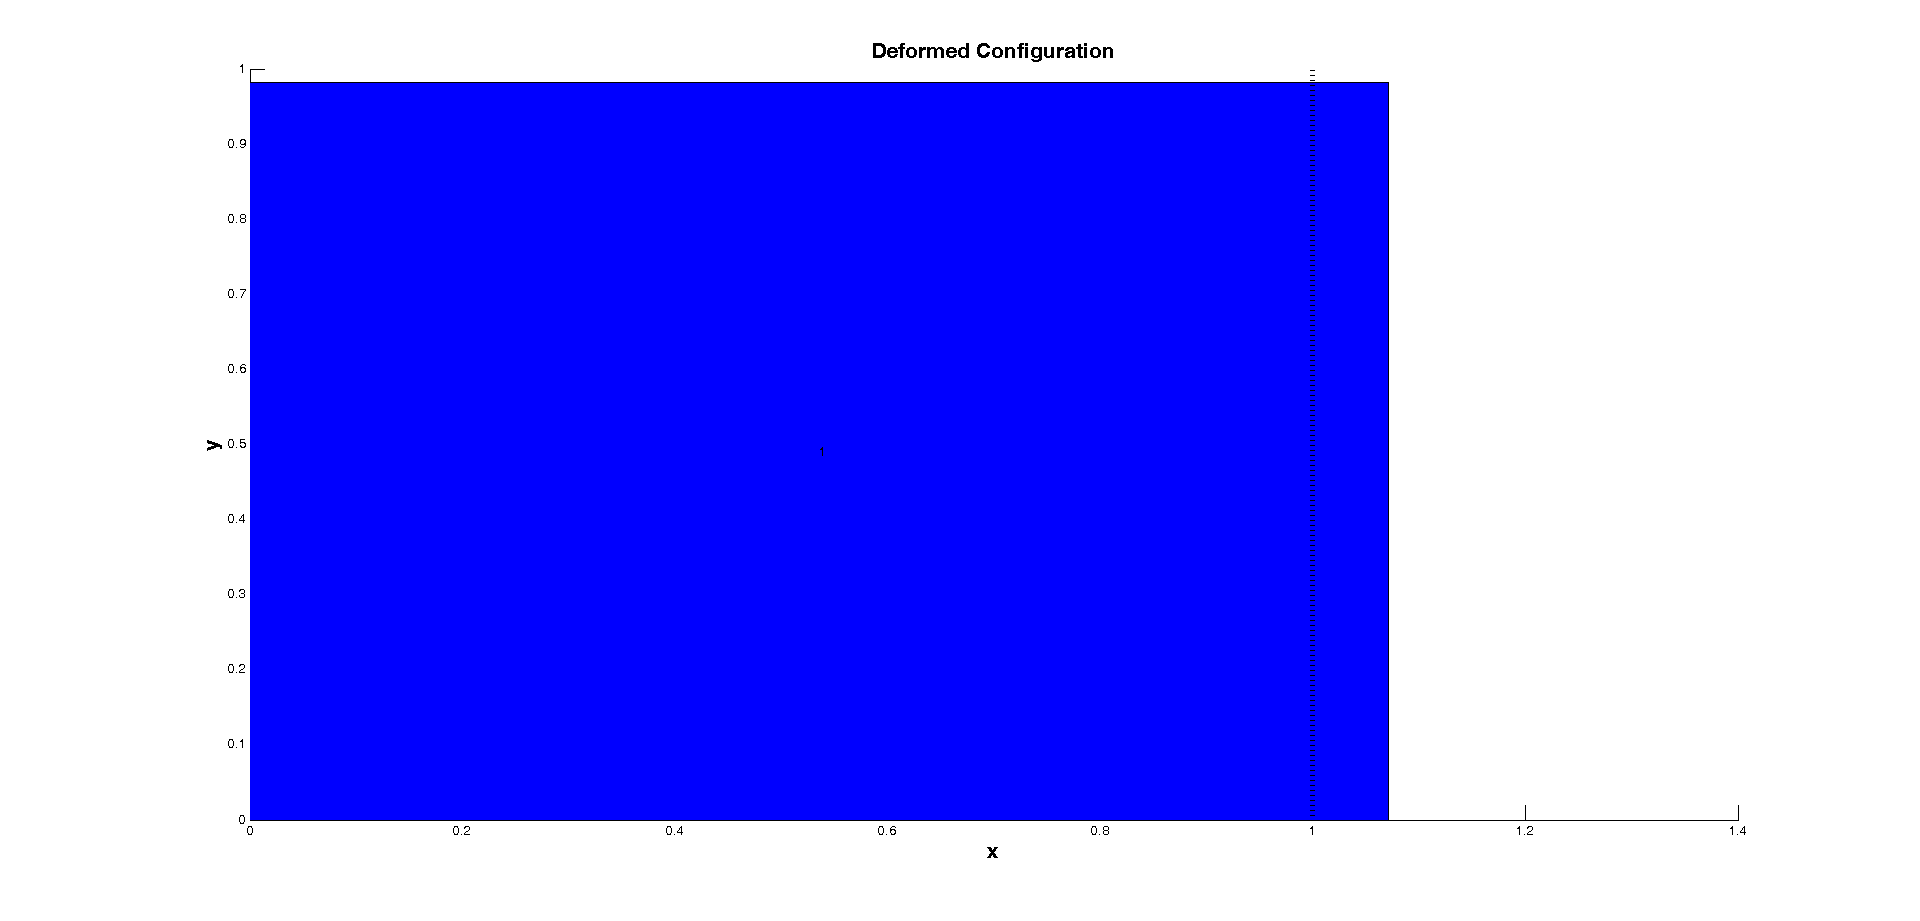
\includegraphics[width=7.5in]{Contour} \nonumber
\end{center}
\label{Deformed geometry}
\begin{center}
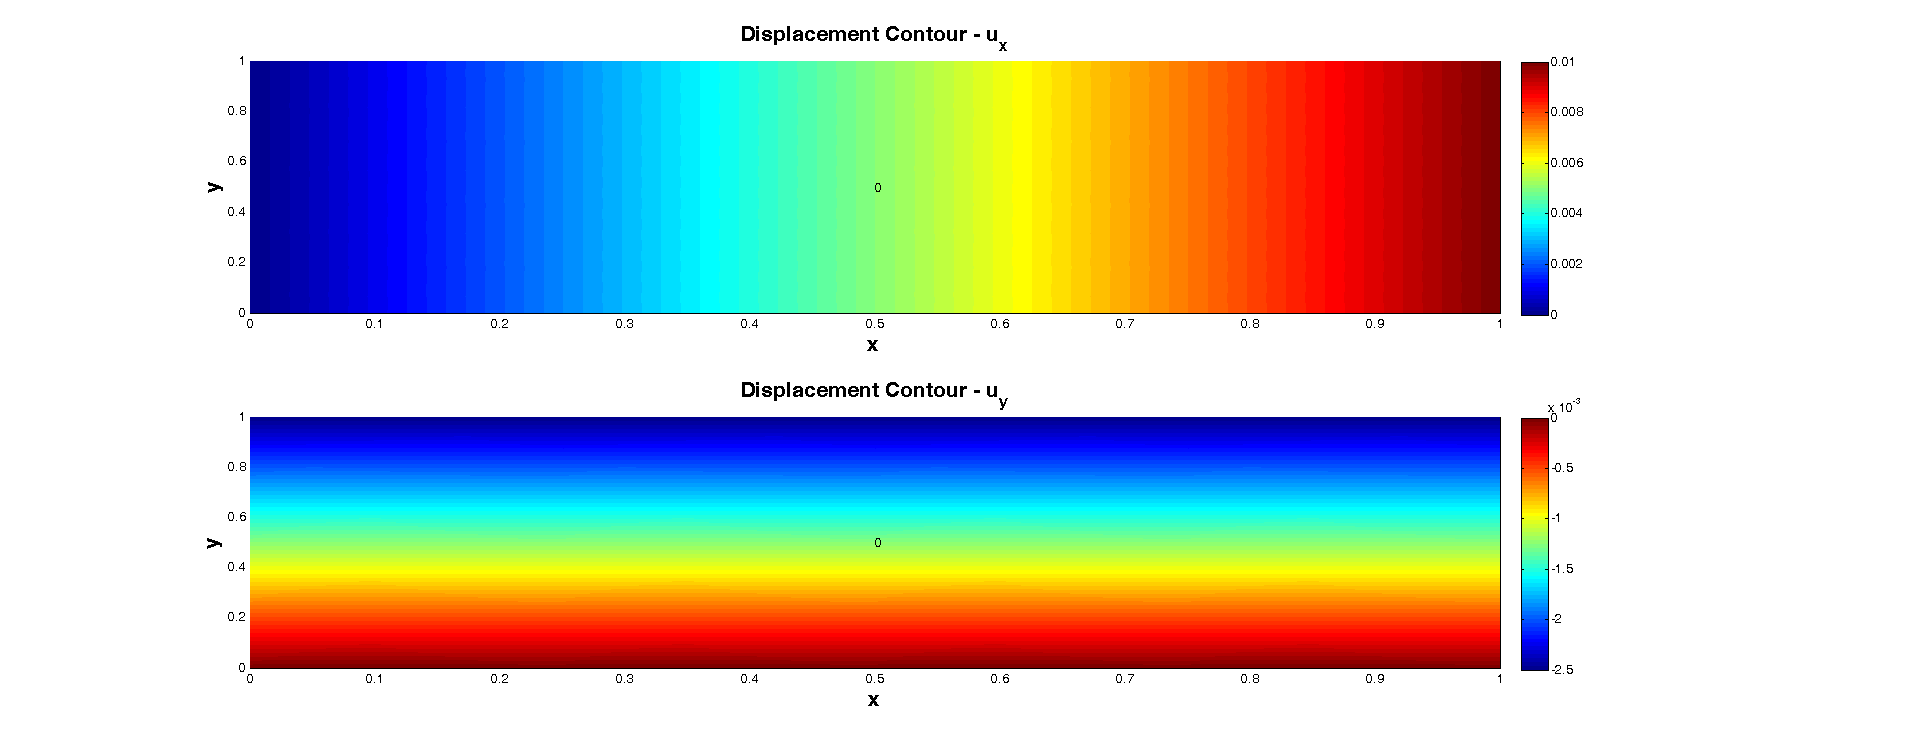
\includegraphics[width=7.5in]{Deformed} \nonumber
\end{center}
\label{Contour}
\newpage
\subsection*{(b) Stress-Strain values}
The values for stresses and strains obtained at the integration points are described below:
\begin{table}[!htbp]
  \centering
  \caption{Stress at Integration points}
    \begin{tabular}{cccc}
    \toprule
    \textbf{Integration Point \textbackslash{}  Stress} & \bf{ $\sigma_{xx}$} & \bf{$\sigma_{yy}$} & \bf{$\sigma_{xy}$} \\
    \midrule
    \textbf{1} & 1 & 4.547E-13 & 0 \\
    \textbf{2} & 1 & 4.547E-13 & 0 \\
    \textbf{3} & 1 & 4.547E-13 & 0 \\
    \textbf{4} & 1 & 4.547E-13 & 0 \\
    \bottomrule
    \end{tabular}%
  \label{tab:addlabel}%
\end{table}%
\begin{table}[!htbp]
  \centering
  \caption{Strain at Integration Points}
    \begin{tabular}{crrr}
    \toprule
    \textbf{Integration Point \textbackslash{}  Strain} & \multicolumn{1}{c}{\bf{$\epsilon_{xx}$}} & \multicolumn{1}{c}{\bf{$\epsilon_{yy}$}} & \multicolumn{1}{c}{\bf{$\epsilon_{xy}$}} \\
    \midrule
    \textbf{1} & 0.01  & -0.0025 & 0 \\
    \textbf{2} & 0.01  & -0.0025 & 0 \\
    \textbf{3} & 0.01  & -0.0025 & 0 \\
    \textbf{4} & 0.01  & -0.0025 & 0 \\
    \bottomrule
    \end{tabular}%
  \label{tab:addlabel}%
\end{table}%
\begin{table}[!htbp]
  \centering
  \caption{Nodal Displacements}
    \begin{tabular}{rrr}
    \toprule
    \multicolumn{1}{l}{\textbf{Node}} & \multicolumn{1}{l}{\textbf{Ux}} & \multicolumn{1}{l}{\textbf{Uy}} \\
    \midrule
    \textbf{1} & 0     & 0 \\
    \textbf{2} & 0.01  & 0 \\
    \textbf{3} & 0.01  & -0.0025 \\
    \textbf{4} & 0     & -0.0025 \\
    \bottomrule
    \end{tabular}%
  \label{tab:addlabel}%
\end{table}%
\subsection*{Matlab Code:}
\lstset{language=Matlab,%
    %basicstyle=\color{red},
    breaklines=true,%
    morekeywords={matlab2tikz},
    keywordstyle=\color{blue},%
    morekeywords=[2]{1}, keywordstyle=[2]{\color{black}},
    identifierstyle=\color{black},%
    stringstyle=\color{mylilas},
    commentstyle=\color{mygreen},%  
    numbersep=9pt, % this defines how far the numbers are from the text
    emph=[1]{for,end,break},emphstyle=[1]\color{red}, %some words to emphasise
    %emph=[2]{word1,word2}, emphstyle=[2]{style},    
}
\lstinputlisting{triangtwo.m}
\lstset{language=Matlab,%
    %basicstyle=\color{red},
    breaklines=true,%
    morekeywords={matlab2tikz},
    keywordstyle=\color{blue},%
    morekeywords=[2]{1}, keywordstyle=[2]{\color{black}},
    identifierstyle=\color{black},%
    stringstyle=\color{mylilas},
    commentstyle=\color{mygreen},%  
    numbersep=9pt, % this defines how far the numbers are from the text
    emph=[1]{for,end,break},emphstyle=[1]\color{red}, %some words to emphasise
    %emph=[2]{word1,word2}, emphstyle=[2]{style},    
}
\lstinputlisting{CompStrainStress_Elem_Cee570.m}
\lstset{language=Matlab,%
    %basicstyle=\color{red},
    breaklines=true,%
    morekeywords={matlab2tikz},
    keywordstyle=\color{blue},%
    morekeywords=[2]{1}, keywordstyle=[2]{\color{black}},
    identifierstyle=\color{black},%
    stringstyle=\color{mylilas},
    commentstyle=\color{mygreen},%  
    numbersep=9pt, % this defines how far the numbers are from the text
    emph=[1]{for,end,break},emphstyle=[1]\color{red}, %some words to emphasise
    %emph=[2]{word1,word2}, emphstyle=[2]{style},    
}
\lstinputlisting{Elast2d_Elem.m}
\end{document}